\documentclass{article}

\usepackage{amsfonts}
\usepackage{graphicx}
\usepackage{amssymb}
\usepackage{amsmath}
\usepackage{listings}
\usepackage{xcolor}
\usepackage{xparse}

\NewDocumentCommand{\codeword}{v}{%
\texttt{\textcolor{blue}{#1}}%
}

\lstset{language=C,keywordstyle={\bfseries \color{blue}}}


\DeclareMathOperator{\sech}{sech}
\newcommand{\NN}{\mathbb{N}}
\newcommand{\RR}{\mathbb{R}}
\newcommand{\QQ}{\mathbb{Q}}
\newcommand{\ZZ}{\mathbb{Z}}
\newcommand{\dV}{\;\mathrm{d}V}
\newcommand{\dA}{\;\mathrm{d}A}
\newcommand{\dx}{\;\mathrm{d}x}
\newcommand{\dy}{\;\mathrm{d}y}
\newcommand{\dz}{\;\mathrm{d}z}
\newcommand{\cA}{\mathcal{A}}
\newcommand{\Bb}{\mathcal{B}}
\newcommand{\Ww}{\mathcal{W}}
\newcommand{\Dd}{\mathcal{D}}
\newcommand{\Ss}{\mathcal{S}}
\newcommand{\Ee}{\mathcal{E}}
\DeclareMathOperator{\im}{im}

\newcommand{\lskip}{\newpage}


\setlength\parindent{18pt}

\begin{document}

1) Read the assembly code below; add comments to explain what each line of code is doing;
in one sentence, explain what this procedure is trying to accomplish. (15 points) 

\begin{lstlisting}[language={[x86masm]Assembler}]

new-proc:
    sll $a0, $a0, 24
    srl $a0, $a0, 24
    add $v0, $a0, $zero
    jr $ra

\end{lstlisting}


Answer:

\begin{lstlisting}[language={[x86masm]Assembler}]

new-proc:
    sll $a0, $a0, 24  # Shift the contents of register $a0 left by 24 bits.
    # Importantly it inserts zeros.
    srl $a0, $a0, 24  # Shifts the result from the
    # previous operation back to the right by 24 bits.
    add $v0, $a0, $zero  # Adds the content of
    # register $a0 to $zero (which is always 0) and stores the result in $v0.
    jr $ra  # Returns to the address stored
    # in the return address register ($ra).

\end{lstlisting}

This procedure extracts out the lowest 8 bits of the \$a0 register and stores
it in \$v0. It then returns to the caller.


\newpage

2) Read the assembly code below; add comments to explain what each line of code
is doing; provide a simple equation to express the return value v0
as a function of input arguments a0 and a1. (30 points) 

\begin{lstlisting}[language={[x86masm]Assembler}]

new-proc:
    blt $a1, $zero, loop2
loop1:
    beq $a1, $zero, proc-end
    sll $a0, $a0, 1
    addi $a1, $a1, -1
    j loop1
loop2:
    beq $a1, $zero, proc-end
    srl $a0, $a0, 1
    addi $a1, $a1, 1
    j loop2
proc-end:
    add $v0, $a0, $zero
    jr $ra

\end{lstlisting}


Answer:

\begin{lstlisting}[language={[x86masm]Assembler}]

new-proc:
    blt $a1, $zero, loop2  # Branch to loop2 if $a1 is less than 0.
loop1:
    beq $a1, $zero, proc-end  # If $a1 is 0, go to proc-end.
    sll $a0, $a0, 1  # Multiply $a0 by 2.
    addi $a1, $a1, -1  # Decrease $a1 by 1.
    j loop1  # Jump back to the start of loop1.
loop2:
    beq $a1, $zero, proc-end  # If $a1 is 0, go to proc-end.
    srl $a0, $a0, 1  # Divide $a0 by 2.
    addi $a1, $a1, 1  # Increase $a1 by 1.
    j loop2  # Jump back to the start of loop2.
proc-end:
    add $v0, $a0, $zero  # Move the content of $a0 to $v0.
    jr $ra  # Returns to the address stored
    # in the return address register ($ra).

\end{lstlisting}

Equation:

If $a1 \geq 0$, $v0 = a0$ $\cdot$ 2 $^\wedge$ $a1$

If $a1 < 0$, $v0 = a0$ / 2 $^\wedge$ ($-a1$)


\newpage

3)  For the (pseudo) assembly code below, replace X, Y, P, and Q
with the smallest set of instructions to save/restore values on
the stack and update the stack pointer. Assume that procA and
procB were written independently by two different programmers
who are following the MIPS guidelines for caller-saved and
callee-saved registers. In other words, the two programmers
agree on the registers handling input arguments and return
value of procB, but they can't see the code written by the
other person. Assume that \$fp isn't being used by either
procA or procB. Be sure to read the class notes first so
you understand the MIPS guidelines for caller-saved and
callee-saved registers. (40 points) 


procA:

    \$s0 = ...

    \$s1 = ...

    \$s2 = ...

    \$s3 = ...

    \$t0 = ...

    \$t1 = ...

    \$t2 = ...

    \$t3 = ...

    X

    \$a0 = ...

    \$a1 = ...

    jal procB

    Y

    ... = \$s3

    ... = \$t1

    ... = \$t2

    ... = \$a0 (this is the value that was originally passed to procA as an argument)

    jr \$ra

procB:

    P

    ... = \$a0

    ... = \$a1

    \$s1 = ...

    \$s2 = ...

    \$s3 = ...

    \$t0 = ...

    \$t1 = ...

    Q

    jr \$ra


Answer:

For X:

No caller-saved registers to preserve since procA
does not expect them to be preserved.

For Y:

No need to restore any caller-saved registers as procA
does not expect them to be preserved.

For P:

\begin{lstlisting}[language={[x86masm]Assembler}]

subu $sp, $sp, 12  # Allocate space on the stack for 3 registers.
sw $s1, 0($sp)     # Save $s1 on the stack.
sw $s2, 4($sp)     # Save $s2 on the stack.
sw $s3, 8($sp)     # Save $s3 on the stack.

\end{lstlisting}

For Q:

\begin{lstlisting}[language={[x86masm]Assembler}]

lw $s1, 0($sp)     # Restore $s1 from the stack.
lw $s2, 4($sp)     # Restore $s2 from the stack.
lw $s3, 8($sp)     # Restore $s3 from the stack.
addu $sp, $sp, 12  # Deallocate space on the stack.

\end{lstlisting}


\newpage

4) Download and install the MARS simulator. Read this Google doc before you start.
Create a new file and copy-paste the code below into the Edit window.
Execute the program. The program should print "BOO7" at the bottom.
Take a screenshot of your MARS screen. Annotate this image to show that
one of the registers and one of the memory locations has the integer 7,
and three registers and three memory locations have the ASCII codes for
the three characters "B", "O", and "O". Your annotation can be as
simple as a circle with the corresponding label (7, B, O, O). (15 points)

\begin{lstlisting}[language={[x86masm]Assembler}]

.data

    str: .asciiz "BOO"
    myint: .word 7

.text

    li $v0, 4 # load immediate; 4 is the code for print_string
    la $a0, str # the print_string syscall expects the string
    # address as the argument; la is the instruction
    # to load the address of the operand (str)
    syscall # MARS will now invoke syscall-4.
    # This should print the string on the bottom of the screen.
    lb $t1, ($a0) # load the byte at address $a0 into register $t1
    lb $t2, 1($a0) # load the byte at address $a0+1 into register $t2
    lb $t3, 2($a0) # load the byte at address $a0+2 into register $t3
    li $v0, 1 # syscall-1 corresponds to print_int
    lw $a0, myint # Bring the value at label myint to register $a0.
    # print_int expects the integer to be printed in $a0.
    syscall # MARS will now invoke syscall-1 

\end{lstlisting}


Answer:

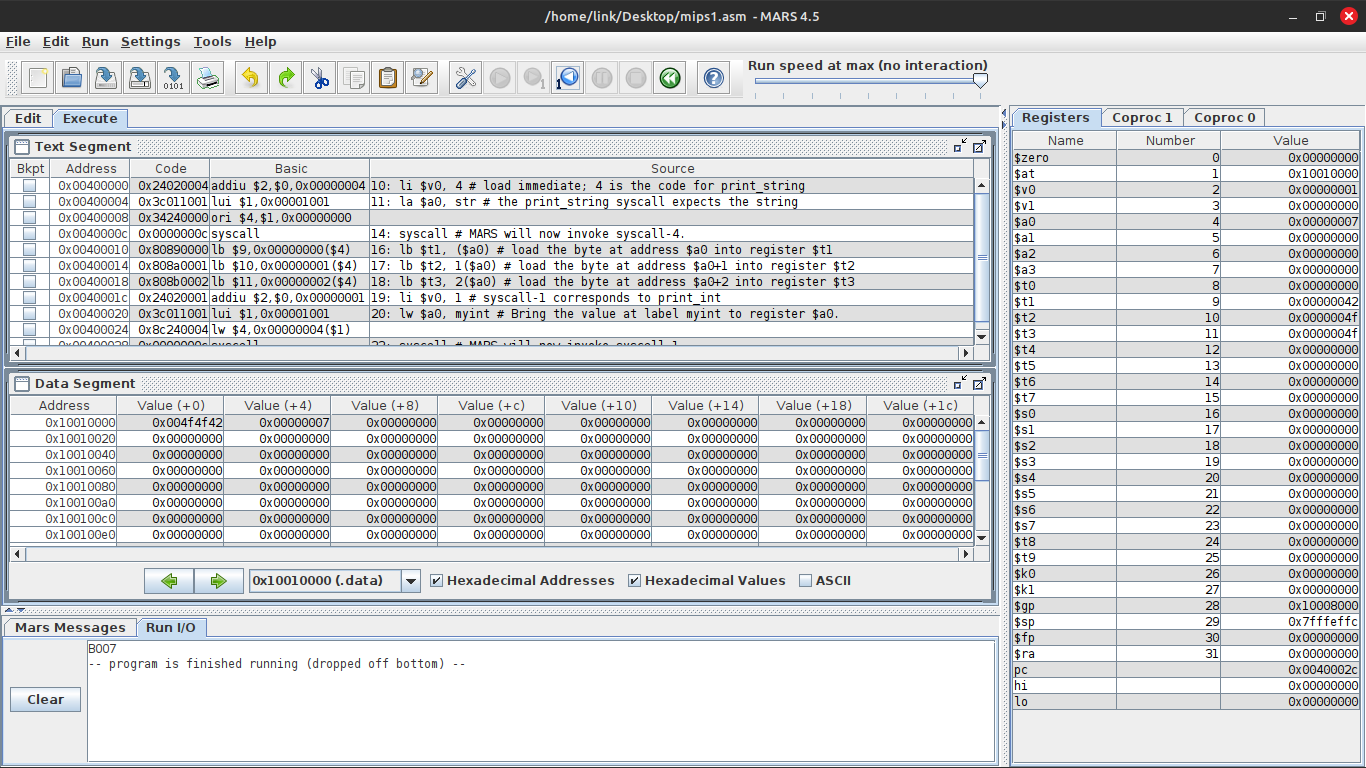
\includegraphics[width=\linewidth]{execution_output}

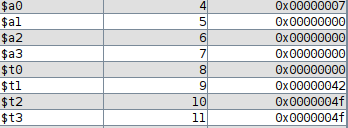
\includegraphics[width=\linewidth]{register_values}

a0 = 7; t0 = 'B'; t2 = 'O'; t3 = 'O'.


\end{document}
